% !TEX encoding = UTF-8
% !TEX TS-program = pdflatex
% !TEX root = ../tesi.tex

%**************************************************************
\chapter{Descrizione dello stage}
\label{cap:processi-metodologie}
%**************************************************************

In questo capitolo viene descritto il modo più dettagliato il progetto dello stage, presentati gli obiettivi e le pianificazioni previste. infine vengono illustrate le tecnologie usate per la realizzazione del progetto. 

%**************************************************************
\section{Il progetto di stage}

L'azienda Sanmarco Informatica S.p.A. fornisce attualmente un servizio di BI per la gestione dei processi di budget. La soluzione attuale si basa su un applicativo web \gls{B2B}. Essendo tale applicativo realizzato con tecnologie poco recenti si è mirato quindi a migliorarlo, aggiornando le tecnologie, mantenendo però la gran parte della struttura esistente invariata.  A questo scopo il team NextBI si è preso l'impegnativa di estenderlo, migliorando le funzionalità esistenti e aggiungendone delle altre nuove, nominando il progetto Budget. In base alla pianificazione, la dimensione di questo progetto risulta molto grande (stimato il rilascio nell'ottobre 2018). Da questa stima si deduce infatti che l'interesse del progetto non si limita solo all'aggiornamento della versione dell'applicativo esistente, ma bensì integrando man mano nel tempo migliorie e servizi innovativi. Il mio progetto si inserisce quindi all'interno del progetto budget con lo scopo di realizzare un sistema portabile e flessibile per la gestione e il monitoraggio di alcuni processi aziendali come sono ad esempio: gli ordini degli articoli giornalieri (settimanali o mensili), la disponibilità, lo spedito, le scadenze, gli inevasi eccetera. Si include anche la necessità di poter notificare l'utente interessato quando un nuovo report è stato aggiunto oppure modificato. 
\\ \\
Il problema che sorge è quindi la mancanza di un sistema portatile e di facile installazione che interroghi il database gestionale, il quale ,in tempo reale fornisca una paginazione aggiornato dei dati d'interesse. Il tutto dovrà essere integrato facilmente nel progetto Budget che si sta sviluppando in parallelo. Lo scopo finale è quindi di avere un sistema robusto e di facile utilizzo che diminuisca i costi di mantenimento del codice. Questo perchè da un'analisi fatta dall'azienda stessa negli ultimi anni i costi di mantenimento dell'applicativo sono  stati significanti.

A questo si aggiunge l'opportunità di includere un sistema di notificazione per gli utenti amministratori quando un utente generico ha chiesto di essere abilitato, ed anche l'opportunità di un miglioramento dell'applicativo preesistente per quanto riguarda  la gestione dell'inserimento e rimozione degli utenti con la profilazione dati per tipo utente.



\begin{table}
\section{Obiettivi}

Gli obiettivi da raggiungere per la durata del progetto dello stage sono classificati in obbligatori e desiderabili con una struttura come segue.

La suddivisione degli obiettivi avviene per tipologia a secondo dell'importanza e vengono numerati in ordine crescente. Vengono rappresentati inoltre da una sigla formata da \textbf{OB-}[numero]-[tipologia]. Il numero è un valore progressivo che identifica l'obiettivo univocamente e la tipologia può essere \textbf{O} oppure \textbf{D} a seconda dell'importanza dell'obiettivo. \\\\

%Gli obiettivi possono essere: \\

%Obbligatori: rappresenta un requisito il cui soddisfacimento è fondamentale
%per raggiungere lo scopo prefissato nel progetto di stage;
%\\\\
%Desiderabili: indica un requisito non necessario per raggiungere gli scopi
%prefissati nel progetto di stage ma che completerebbero maggiormente il risultato finale.
%\\\\





\begin{tabular}{ |p{2cm}|p{3cm}|p{8cm}| }

 \hline
\textbf{ ID}   &  \textbf{IMPORTANZA}    &  \textbf{DESCRIZIONE} \\ 

 \hline
  OB-1-O &  Obbligatorio   & Studio e disegno del database per la permanenza dei dati che riguardano la gestione degli utenti, delle licenze e la gestione della tastiera Telegram.\\
 \hline
OB-2-O &   Obbligatorio  &  Acquisizione dati dal database gestionale, elaborazione  e scrittura dati ETL \\
 \hline
 OB-3-O &   Obbligatorio  &  Associazione utente B2B con l'utente telegram \\
 \hline
 OB-4-O & Obbligatorio & Gestione di profilazione delle reporistiche in base all'utente telegram.\\
\hline
OB-5-O  & Obbligatorio & Creazione tabelle per le reporistiche in vari formati richiesti. \\
\hline
OB-6-O  &  Obbligatorio  & Gestione attivazione utente generico da un amministratore. Gestione di inserimento e rimozione degli utenti generici da parte dell'utente amministratore.\\
\hline  
OB-7-O & Obbligatorio & Gestione delle licenze, rimozione e prolungamenti delle stesse. \\
\hline
OB-8-O & Obbligatorio & Gestione lista utenti in attesa . \\
\hline
OB-9-D & Desiderabile & Test per le formule riassuntive dell'applicativo preesistente. \\
\hline
OB-10-D & Desiderabile & Integrazione della documentazione con quella  dell'applicativo preesistente con eventuali aggiunte di diagrammi dei casi d'uso. \\
\hline

\end{tabular}
\\\\
\caption{Tabella degli obiettivi}
\end{table}


%Nel capito Conclusioni al paragrafo (?) "Raggiungimento degli obiettivi", viene presentato il livello di soddisfacimento degli obiettivi a consuntivo.


\clearpage
\section{Vincoli}
Per l'esecuzione dello stage presso Sanmarco Informatica S.p.A sono stati fissati alcuni vincoli: 

\begin{itemize}

\item Per facilitare l'integrazione nel progetto Budget, l'applicativo è stato richiesto di essere sviluppato in Java mantenendo così una certa compatibilità con la piattaforma di base del progetto Budget. 

\item Un altro vincolo è quello di usare il sistema ETL (Extract, Transform, Load) per estrarre e trasformare i dati dal database gestionale in un altro database che comunicherà direttamente con il nostro applicativo. Questo vincolo è dovuto dal fatto che non è consentito effettuare delle modifiche direttamente al database gestionale dell'azienda.

\item Un altro criterio da rispettare è stato l'uso  dell'\gls{IDE} Eclipse Neon per la scrittura e la compilazione del codice sorgente.

 \item E' stato inoltre richiesto di usare RTC (Rational Team Concert), integrato nell'IDE eclipse per gestire la parte di versionamento del codice. Il tutor aziendale attraverso l'RTC si impegnava ad assegnare gli sprint per una certa attività con una durata non maggiore di tre settimane. 
 
 Per la parte di pianificazione e gestione delle attività invece, è stato richiesto di usare Asana.  
 
 \end{itemize}

\clearpage

\begin{table}
\section{Pianificazione}

Per la pianificazione dello stage è stato suddiviso il lavoro in diverse attività assegnando una durata temporale idonea, tenendo conto dei limiti di tempo previsti di massimo 308 ore. Lo stage è stato suddiviso nelle seguenti attività: \\

\begin{tabular}{ |p{3cm}|p{1cm}|p{8cm}| }

 \hline
\textbf{Attività}   &  \textbf{Ore}    &  \textbf{DESCRIZIONE} \\ 

 \hline
  Studio introduttivo delle tecnologi principali coinvolte &  64 & Studio e la configurazione di Eclipse con tutti i suoi \gls{plug-in} necessari per avviare il progetto. Lo studio del tool DBeaver che è stato utilizzato per l'organizzazione e la gestione della base di dati e lo studio dell'architettura di base dell'applicativo con i suoi servizi da implementare.\\
 \hline
Studio di fattibilità per la realizzazione del sistema &   25  & Studio di fattibilità per capire se sia effettivamente possibile fornire un sistema sempre a portata di mano, robusto e dinamico, capace di fornire le funzionalità  presenti nell'applicativo preesistente. \\
 \hline
 Analisi dei requisiti &   30  & Questa periodo rappresenta uno studio delle funzionalità che il software dovrebbe soddisfare per essere considerato funzionale dall'azienda. \\
 \hline
  Progettazione dell'architettura &   70  & Studio della progettazione architetturale. Studio di come saranno effettuate le query sul Data Base Postgres e come saranno presentati i dati elaborati sull'interfaccia front-end.  \\
 \hline
   Implementazione del sistema &   65  & Acquisizione dati con successiva scrittura attraverso ETL e l'implementazione dei servizi back-end che si occuperanno di riportare in modo efficiente ed efficace i dati richiesti dall'utente. Un aspetto importante in questo processo è quello di tener conto dei tempi di risposta al lato client.  \\
 \hline
   Test e sperimentazione del sistema &   24  & In questo periodo si prosegue con i test di correttezza e validazione del sistema e delle modifiche apportate per assicurare che rispettino le aspettative previste.  \\
 \hline
    Documentazione&   30  & Questo  processo comprende l'intera attività di documentazione effettuata durante il periodo di stage. Al contrario delle altre, questa è un'attività trasversale che riguarda in parte ogni altra attività e continua per l'intera durata dello stage.  \\
 \hline

\end{tabular}
\\\\
\caption{Tabella della pianificazione}
\end{table}




 \clearpage
\begin{figure}[h!]
\section{Ambiente di lavoro}
\begin{center}
    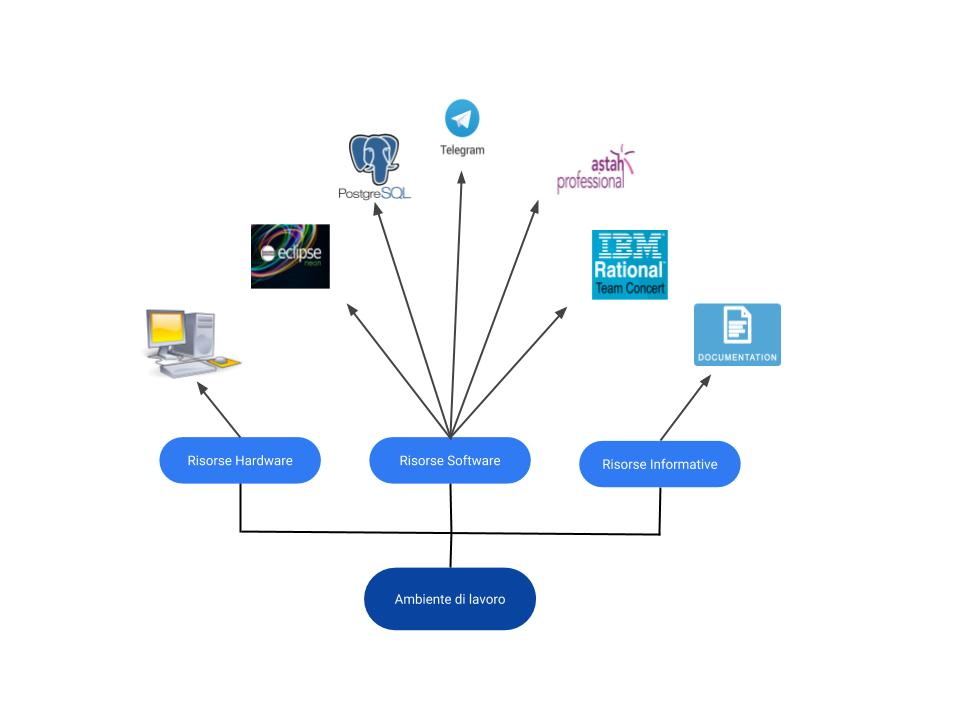
\includegraphics[scale=0.43]{ambiente_di_lavoro} 
    \caption{Ambiente di lavoro}
    \end{center}
 All'inizio dell'attività di stage, dall'azienda Sanmarco Informatica S.p.A. ho avuto accesso a diverse risorse dell'azienda per permettermi di eseguire il lavoro al meglio. \\
Le risorse condivise dall'azienda si suddividono in risorse hardware e risorse software, con i programmi messi a disposizione dall'azienda, e risorse informative, che comprendono i materiali di studio forniti inizialmente dall'azienda. 
\end{figure}  



\subsection{Risorse hardware}

Il team NextBI che fa parte nell'ambiente di Ricerca e Sviluppo dell'azienda Sanmarco Informatica S.p.A. mi ha seguito durante lo stage rendendomi il lavoro più facile con la loro collaborazione e disponibilità di formazione. \\

Mi è stato consegnato un PC aziendale già configurato con gli ambienti di lavoro aggiornati e alcuni software preinstallati per facilitare la fase di configurazione dell'ambiente. \\
Oltre al PC aziendale, mi è stato consentito l'utilizzo di una macchina virtuale per effettuare dei test necessari, molto utile soprattutto per l'esecuzione di ETL che richiedono tempi di esecuzione molto lunghi. 
\subsection{Risorse software}
Ho avuto accesso al repository aziendale basato su RTC il quale gestisce il versionamento del codice. I'RTC è stato configurato con l'IDE di Eclipse per garantire la compatibilità del sistema di versionamento già present nell'applicativo preesistente. \\
Il PC aziendale inoltre, aveva preinstallato la maggior parte dei software utili per effettuare il lavoro con versioni aggiornati. \\\\
Inoltre mi è stato consentito installare anche nuovi software, tools o librerie se necessari, a volte utili in particolari circostanze.

\subsection{Risorse informative}
Mi sono state fornite diverse risorse informative tra cui diverse note, manuali di programmazione  e la relativa documentazione dell'applicativo preesistente nel quale si va ad integrare il progetto di stage. Quest'ultimo ha favorito l'apprendimento corretto del funzionamento dell'applicativo preesistente a fine di ammortizzare i tempi di progettazione. 

\section{Tecnologie usate}
Sono varie le tecnologie usate durante lo stage. In questo paragrafo vengono descritte le diverse tecnologie usate con una breve presentazione. \\\\

\begin{enumerate}

\item \textbf{Java: }Java è un linguaggio di programmazione ad alto livello, orientato agli oggetti e a tipizzazione statica, specificatamente progettato per essere il più possibile indipendente dalla piattaforma di esecuzione.\\
La sua semplicità unita all'essere un linguaggio multi piattaforma lo rende molto usato e fa si che disponga di un'elevata quantità di librerie facilmente integrabili per le attività varie.\\
Uno dei principi fondamentali del linguaggio Java è espresso dal motto WORA (write once, run anywhere, ossia "scrivi una volta, esegui ovunque"): il codice compilato che viene eseguito su una piattaforma non deve essere ricompilato per essere eseguito su una piattaforma diversa. Il prodotto della compilazione è infatti in un formato chiamato bytecode che può essere eseguito da una qualunque implementazione di un processore virtuale detto Java Virtual Machine. 
Al 2014, Java risulta essere uno dei linguaggi di programmazione più usati al mondo, specialmente per applicazioni client-server, con un  numero di sviluppatori stimato intorno ai 9 milioni.\\\\

\item \textbf{XML (Extensible Markup Language) : }XML è un linguaggio di markup che definisce regole per la codifica di documenti in un formato comprensibile sia se letto da un umano che da una macchina. Lo scopo principale del formato è concentrato sulla semplicità, generalità e usabilità generale. Il formato permette quindi di definire tag personalizzati per i vari campi e mantenere un output che sia analizzabile in maniera automatica e manuale.
Il formato è stato usato perchè già integrato all'interno del Plug-in MyBatis per generare gli oggetti DAO corrispondenti alle tabelle del database.

\item \textbf{PostgresSQL :}
PostgreSQL è un completo modello di base di dati (\gls{DBMS}) ad oggetti rilasciato con licenza libera (stile Licenza BSD).\\
PostgreSQL è una reale alternativa sia rispetto ad altri prodotti liberi come MySQL, Firebird SQL che a quelli a codice chiuso come Oracle, IBM o DB2 ed offre caratteristiche uniche nel suo genere che lo pongono per alcuni aspetti all'avanguardia nel settore dei database.\\
PostgresSQL è stato utile nel progetto poichè ha permesso di collegare diversi database e farli comunicare tra loro con un'interfaccia facile da manovrare.\\
PostgreSQL, inoltre, permette l'ereditarietà dei tipi, uno dei principali concetti della programmazione orientata agli oggetti\\
Infine, con PostgreSQL si può implementare la logica in uno dei molti linguaggi supportati.

\item \textbf{Notepad++ : } Notepad++ è un text editor \gls{open source} mirato alla modifica di codice sorgente. Il programma non dispone di tutte le capacità di un vero IDE ma presenta funzionalità più basilari come syntax highlighting (evidenziazione della sintassi) per 
vari linguaggi tra cui anche Java, ricerca avanzata anche tramite espressioni regolari e la possibilità di aggiungere diversi plugin per espanderne le capacità.
Notepad++ si è rivelato molto utile sia come semplice text editor ma anche per permettere rapide modifiche al codice grazie alla maggiore rapidità presentata rispetto a Eclisse.

\item \textbf{Astah Community Astah Community: } Astah è un programma per la modellazione di schemi UML (Unified Modeling Language) cioè rispettanti degli standard industriali per i modelli general-purpose per l'ingegneria del software.
Il programma è stato scelto perchè ritenuto abbastanza semplice da usare per lo scopo necessario dopo esperienze precedenti ed è stato usato per creare alcuni diagrammi durante la fase di progettazione.

\item \textbf{Evernote :} Evernote è un programma multi piattaforma mirato alla creazione di note, la loro organizzazione, archiviazione e condivisione. Dispone sia di client installabile sia di un'interfaccia web e permette anche di condividere piccoli file.
L'uso del programma è stato richiesto da parte del tutor ed è servito per parte del processo di documentazione. Su di esso sono stati infatti tenute cronologie, appunti e tracce delle decisioni che sono state fatte man mano durante il proseguimento dello stage.

\item \textbf{Visual Studio Code :}
Visual Studio Code è un editor di codice sorgente sviluppato da Microsoft compatibile cin diversi sistemi operativi.
Visual Studio Code è basato su Electron, un \gls{framework} con cui è possibile sviluppare applicazioni Node.js.\\
Questo editor supporta vari linguaggi di programmazione, tra cui anche JavaScript e Java.
Visual Studio Code permette installare varie estensioni, con la possibilità di fare ciò direttamente dal programma. \\
Il software Visual Studio è stato usato principalmente per facilitare lo sviluppo front-end grazie alle sue numerose estensioni disponibili facilmente instancabili. 

\item \textbf{Telegram :} Telegram è un servizio di messaggistica istantanea basato su cloud ed erogato senza fini di lucro dalla società Telegram LLC. I client ufficiali di Telegram sono distribuiti come software libero per diverse piattaforme. \\\\
Da giugno 2015 Telegram ha introdotto una piattaforma per permettere, a sviluppatori terzi, di creare i Bot. I Bot sono degli account Telegram, gestiti da un programma, che offrono molteplici funzionalità con risposte immediate e completamente automatizzate. Grazie a questa funzionalità, il Bot telegrma è diventata la piattaforma dove si basa la maggior parte dell'applicativo sviluppato durante il periodo dello stage.

\item \textbf{FileZilla :} FileZilla Client è un software libero multipiattaforma che permette il trasferimento di file in Rete attraverso il protocollo FTP. Il programma è disponibile per GNU/Linux, Microsoft Windows, e macOS. Tra i vari protocolli supportati, oltre all'FTP vi è l'SFTP, e l'FTP su SSL/TLS. 
Il codice sorgente di FileZilla è disponibile sul sito SourceForge e, in alcuni casi, anche al momento dell'installazione del programma. Il progetto fu nominato Progetto del Mese nel novembre del 2003.\\
Questo software è stato usato nel periodo dello stage per poter permettere dei trasferimenti di diversi file dal server dell'azienda Sanmarco Informatica a quello dei clienti dove è stato installata la demo. \\


\end{enumerate} 






















